\documentclass{standalone}
\usepackage{tikz}
\usetikzlibrary{patterns, positioning}


\begin{document}
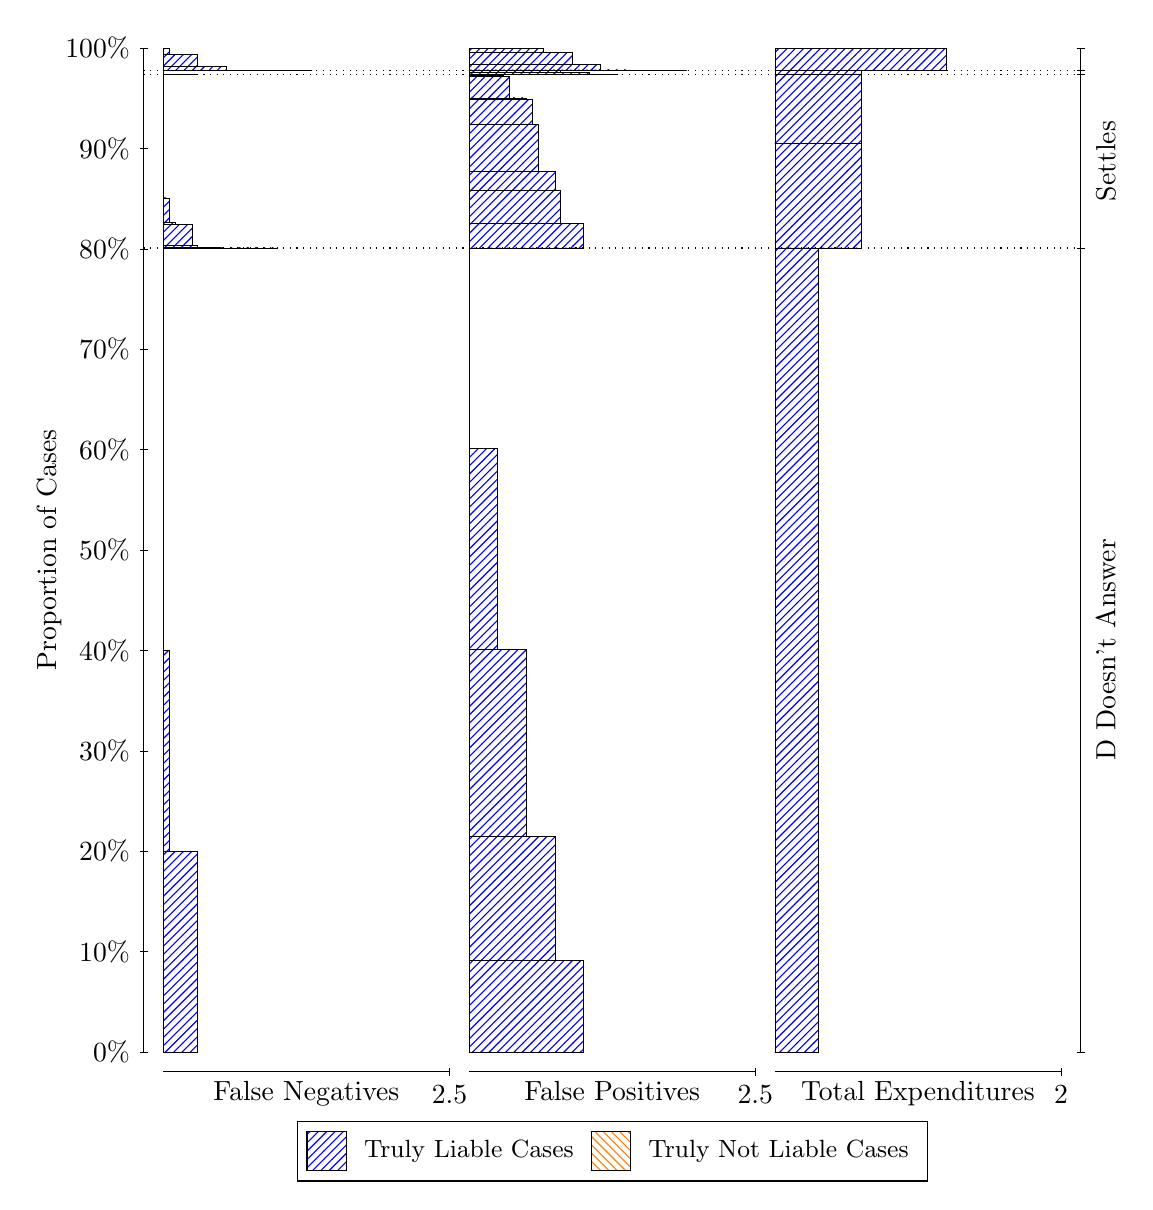
\begin{tikzpicture}
\draw[black, very thin] (1.5,1.75) -- (1.5,14.5);
\node[rotate=90, text=black, anchor=center] at (0.3, 8.125) {Proportion of Cases};
\draw[black, very thin] (1.45,1.75) -- (1.55,1.75);
\node[text=black, anchor=east] at (1.45, 1.75) {0\%};
\draw[black, very thin] (1.45,3.025) -- (1.55,3.025);
\node[text=black, anchor=east] at (1.45, 3.025) {10\%};
\draw[black, very thin] (1.45,4.3) -- (1.55,4.3);
\node[text=black, anchor=east] at (1.45, 4.3) {20\%};
\draw[black, very thin] (1.45,5.575) -- (1.55,5.575);
\node[text=black, anchor=east] at (1.45, 5.575) {30\%};
\draw[black, very thin] (1.45,6.85) -- (1.55,6.85);
\node[text=black, anchor=east] at (1.45, 6.85) {40\%};
\draw[black, very thin] (1.45,8.125) -- (1.55,8.125);
\node[text=black, anchor=east] at (1.45, 8.125) {50\%};
\draw[black, very thin] (1.45,9.4) -- (1.55,9.4);
\node[text=black, anchor=east] at (1.45, 9.4) {60\%};
\draw[black, very thin] (1.45,10.675) -- (1.55,10.675);
\node[text=black, anchor=east] at (1.45, 10.675) {70\%};
\draw[black, very thin] (1.45,11.95) -- (1.55,11.95);
\node[text=black, anchor=east] at (1.45, 11.95) {80\%};
\draw[black, very thin] (1.45,13.225) -- (1.55,13.225);
\node[text=black, anchor=east] at (1.45, 13.225) {90\%};
\draw[black, very thin] (1.45,14.5) -- (1.55,14.5);
\node[text=black, anchor=east] at (1.45, 14.5) {100\%};

\draw[black, very thin] (13.4,1.75) -- (13.4,14.5);
\draw[black, very thin] (13.35,1.75) -- (13.45,1.75);
\node[anchor=west] at (13.35, 1.75) {};
\draw[black, very thin] (13.35,11.961) -- (13.45,11.961);
\node[anchor=west] at (13.35, 11.961) {};
\draw[black, very thin] (13.35,14.167) -- (13.45,14.167);
\node[anchor=west] at (13.35, 14.167) {};
\draw[black, very thin] (13.35,14.214) -- (13.45,14.214);
\node[anchor=west] at (13.35, 14.214) {};
\draw[black, very thin] (13.35,14.5) -- (13.45,14.5);
\node[anchor=west] at (13.35, 14.5) {};

\draw[black, very thin, pattern color=blue, pattern=north east lines] (1.75,1.75) rectangle (2.186,4.2999);
\draw[black, very thin, pattern color=blue, pattern=north east lines] (1.75,4.2999) rectangle (1.8227,6.8485);
\draw[black, very thin, pattern color=orange, pattern=north west lines] (1.75,6.8485) rectangle (1.75,6.8485);
\draw[black, very thin, pattern color=blue, pattern=north east lines] (1.75,6.8485) rectangle (1.75,11.961);
\draw[black, very thin, pattern color=blue, pattern=north east lines] (1.75,11.961) rectangle (3.2033,11.961);
\draw[black, very thin, pattern color=blue, pattern=north east lines] (1.75,11.961) rectangle (2.9127,11.961);
\draw[black, very thin, pattern color=blue, pattern=north east lines] (1.75,11.961) rectangle (2.84,11.961);
\draw[black, very thin, pattern color=blue, pattern=north east lines] (1.75,11.961) rectangle (2.622,11.961);
\draw[black, very thin, pattern color=blue, pattern=north east lines] (1.75,11.961) rectangle (2.5493,11.961);
\draw[black, very thin, pattern color=blue, pattern=north east lines] (1.75,11.961) rectangle (2.4767,11.971);
\draw[black, very thin, pattern color=blue, pattern=north east lines] (1.75,11.971) rectangle (2.2587,11.971);
\draw[black, very thin, pattern color=blue, pattern=north east lines] (1.75,11.971) rectangle (2.186,11.993);
\draw[black, very thin, pattern color=blue, pattern=north east lines] (1.75,11.993) rectangle (2.1133,12.26);
\draw[black, very thin, pattern color=blue, pattern=north east lines] (1.75,12.26) rectangle (1.8953,12.283);
\draw[black, very thin, pattern color=blue, pattern=north east lines] (1.75,12.283) rectangle (1.8227,12.596);
\draw[black, very thin, pattern color=orange, pattern=north west lines] (1.75,12.596) rectangle (1.75,12.596);
\draw[black, very thin, pattern color=blue, pattern=north east lines] (1.75,12.596) rectangle (1.75,14.167);
\draw[black, very thin, pattern color=blue, pattern=north east lines] (1.75,14.167) rectangle (2.186,14.167);
\draw[black, very thin, pattern color=blue, pattern=north east lines] (1.75,14.167) rectangle (1.8227,14.167);
\draw[black, very thin, pattern color=orange, pattern=north west lines] (1.75,14.167) rectangle (1.75,14.167);
\draw[black, very thin, pattern color=blue, pattern=north east lines] (1.75,14.167) rectangle (1.75,14.214);
\draw[black, very thin, pattern color=blue, pattern=north east lines] (1.75,14.214) rectangle (3.6393,14.214);
\draw[black, very thin, pattern color=blue, pattern=north east lines] (1.75,14.214) rectangle (3.276,14.214);
\draw[black, very thin, pattern color=blue, pattern=north east lines] (1.75,14.214) rectangle (2.9127,14.216);
\draw[black, very thin, pattern color=blue, pattern=north east lines] (1.75,14.216) rectangle (2.5493,14.269);
\draw[black, very thin, pattern color=blue, pattern=north east lines] (1.75,14.269) rectangle (2.186,14.269);
\draw[black, very thin, pattern color=blue, pattern=north east lines] (1.75,14.269) rectangle (2.186,14.422);
\draw[black, very thin, pattern color=blue, pattern=north east lines] (1.75,14.422) rectangle (1.8227,14.422);
\draw[black, very thin, pattern color=blue, pattern=north east lines] (1.75,14.422) rectangle (1.8227,14.493);
\draw[black, very thin, pattern color=orange, pattern=north west lines] (1.75,14.493) rectangle (1.75,14.493);
\draw[black, very thin, pattern color=blue, pattern=north east lines] (1.75,14.493) rectangle (1.75,14.5);
\draw[black, very thin, pattern color=orange, pattern=north west lines] (5.6333,1.75) rectangle (7.0867,1.75);
\draw[black, very thin, pattern color=blue, pattern=north east lines] (5.6333,1.75) rectangle (7.0867,2.9133);
\draw[black, very thin, pattern color=blue, pattern=north east lines] (5.6333,2.9133) rectangle (6.7233,4.4867);
\draw[black, very thin, pattern color=blue, pattern=north east lines] (5.6333,4.4867) rectangle (6.36,6.8629);
\draw[black, very thin, pattern color=blue, pattern=north east lines] (5.6333,6.8629) rectangle (5.9967,9.4114);
\draw[black, very thin, pattern color=blue, pattern=north east lines] (5.6333,9.4114) rectangle (5.6333,11.961);
\draw[black, very thin, pattern color=orange, pattern=north west lines] (5.6333,11.961) rectangle (7.0867,11.961);
\draw[black, very thin, pattern color=blue, pattern=north east lines] (5.6333,11.961) rectangle (7.0867,12.27);
\draw[black, very thin, pattern color=orange, pattern=north west lines] (5.6333,12.27) rectangle (6.796,12.27);
\draw[black, very thin, pattern color=blue, pattern=north east lines] (5.6333,12.27) rectangle (6.796,12.688);
\draw[black, very thin, pattern color=blue, pattern=north east lines] (5.6333,12.688) rectangle (6.7233,12.929);
\draw[black, very thin, pattern color=orange, pattern=north west lines] (5.6333,12.929) rectangle (6.5053,12.929);
\draw[black, very thin, pattern color=blue, pattern=north east lines] (5.6333,12.929) rectangle (6.5053,13.532);
\draw[black, very thin, pattern color=blue, pattern=north east lines] (5.6333,13.532) rectangle (6.4327,13.846);
\draw[black, very thin, pattern color=blue, pattern=north east lines] (5.6333,13.846) rectangle (6.36,13.868);
\draw[black, very thin, pattern color=blue, pattern=north east lines] (5.6333,13.868) rectangle (6.142,14.135);
\draw[black, very thin, pattern color=blue, pattern=north east lines] (5.6333,14.135) rectangle (6.0693,14.158);
\draw[black, very thin, pattern color=blue, pattern=north east lines] (5.6333,14.158) rectangle (5.9967,14.158);
\draw[black, very thin, pattern color=blue, pattern=north east lines] (5.6333,14.158) rectangle (5.7787,14.167);
\draw[black, very thin, pattern color=blue, pattern=north east lines] (5.6333,14.167) rectangle (5.706,14.167);
\draw[black, very thin, pattern color=blue, pattern=north east lines] (5.6333,14.167) rectangle (5.6333,14.167);
\draw[black, very thin, pattern color=orange, pattern=north west lines] (5.6333,14.167) rectangle (7.5227,14.167);
\draw[black, very thin, pattern color=blue, pattern=north east lines] (5.6333,14.167) rectangle (7.5227,14.167);
\draw[black, very thin, pattern color=blue, pattern=north east lines] (5.6333,14.167) rectangle (7.1593,14.187);
\draw[black, very thin, pattern color=blue, pattern=north east lines] (5.6333,14.187) rectangle (6.796,14.213);
\draw[black, very thin, pattern color=blue, pattern=north east lines] (5.6333,14.213) rectangle (6.4327,14.214);
\draw[black, very thin, pattern color=blue, pattern=north east lines] (5.6333,14.214) rectangle (6.0693,14.214);
\draw[black, very thin, pattern color=orange, pattern=north west lines] (5.6333,14.214) rectangle (8.3947,14.214);
\draw[black, very thin, pattern color=blue, pattern=north east lines] (5.6333,14.214) rectangle (8.3947,14.214);
\draw[black, very thin, pattern color=orange, pattern=north west lines] (5.6333,14.214) rectangle (8.0313,14.214);
\draw[black, very thin, pattern color=blue, pattern=north east lines] (5.6333,14.214) rectangle (8.0313,14.214);
\draw[black, very thin, pattern color=orange, pattern=north west lines] (5.6333,14.214) rectangle (7.668,14.214);
\draw[black, very thin, pattern color=blue, pattern=north east lines] (5.6333,14.214) rectangle (7.668,14.221);
\draw[black, very thin, pattern color=orange, pattern=north west lines] (5.6333,14.221) rectangle (7.3047,14.221);
\draw[black, very thin, pattern color=blue, pattern=north east lines] (5.6333,14.221) rectangle (7.3047,14.292);
\draw[black, very thin, pattern color=orange, pattern=north west lines] (5.6333,14.292) rectangle (6.9413,14.292);
\draw[black, very thin, pattern color=blue, pattern=north east lines] (5.6333,14.292) rectangle (6.9413,14.444);
\draw[black, very thin, pattern color=blue, pattern=north east lines] (5.6333,14.444) rectangle (6.578,14.498);
\draw[black, very thin, pattern color=blue, pattern=north east lines] (5.6333,14.498) rectangle (6.2147,14.5);
\draw[black, very thin, pattern color=blue, pattern=north east lines] (5.6333,14.5) rectangle (5.8513,14.5);
\draw[black, very thin, pattern color=blue, pattern=north east lines] (5.6333,14.5) rectangle (5.6333,14.5);
\draw[black, very thin, pattern color=orange, pattern=north west lines] (9.5167,1.75) rectangle (10.062,1.75);
\draw[black, very thin, pattern color=blue, pattern=north east lines] (9.5167,1.75) rectangle (10.062,11.961);
\draw[black, very thin, pattern color=orange, pattern=north west lines] (9.5167,11.961) rectangle (10.607,11.961);
\draw[black, very thin, pattern color=blue, pattern=north east lines] (9.5167,11.961) rectangle (10.607,13.288);
\draw[black, very thin, pattern color=orange, pattern=north west lines] (9.5167,13.288) rectangle (10.607,13.288);
\draw[black, very thin, pattern color=blue, pattern=north east lines] (9.5167,13.288) rectangle (10.607,14.167);
\draw[black, very thin, pattern color=orange, pattern=north west lines] (9.5167,14.167) rectangle (10.607,14.167);
\draw[black, very thin, pattern color=blue, pattern=north east lines] (9.5167,14.167) rectangle (10.607,14.214);
\draw[black, very thin, pattern color=orange, pattern=north west lines] (9.5167,14.214) rectangle (11.697,14.214);
\draw[black, very thin, pattern color=blue, pattern=north east lines] (9.5167,14.214) rectangle (11.697,14.5);
\draw[black, dotted] (1.5,11.961) -- (13.4,11.961);
\draw[black, dotted] (1.5,14.167) -- (13.4,14.167);
\draw[black, dotted] (1.5,14.214) -- (13.4,14.214);
\draw[black, very thin] (1.75,1.5) -- (5.3833,1.5);
\node[text=black, anchor=north] at (3.5667, 1.5) {False Negatives};
\draw[black, very thin] (5.3833,1.45) -- (5.3833,1.55);
\node[text=black, anchor=north] at (5.3833, 1.45) {2.5};

\draw[black, very thin] (5.6333,1.5) -- (9.2667,1.5);
\node[text=black, anchor=north] at (7.45, 1.5) {False Positives};
\draw[black, very thin] (9.2667,1.45) -- (9.2667,1.55);
\node[text=black, anchor=north] at (9.2667, 1.45) {2.5};

\draw[black, very thin] (9.5167,1.5) -- (13.15,1.5);
\node[text=black, anchor=north] at (11.333, 1.5) {Total Expenditures};
\draw[black, very thin] (13.15,1.45) -- (13.15,1.55);
\node[text=black, anchor=north] at (13.15, 1.45) {2};

\node[text=black, centered, rotate=90] at (13.72, 6.8557) {D Doesn't Answer};
\node[text=black, centered, rotate=90] at (13.72, 13.064) {Settles};



\draw (7.449999999999999,1.5) node[draw=none] (baseCoordinate) {};
\begin{scope}[align=center]
        \matrix[scale=0.5, draw=black, below=0.5cm of baseCoordinate, nodes={draw}, column sep=0.1cm]{
            \node[rectangle, draw, minimum width=0.5cm, minimum height=0.5cm, pattern color=blue, pattern=north east lines] {}; &
            \node[draw=none, font=\small, text=black] (B) {Truly Liable Cases}; &
            \node[rectangle, draw, minimum width=0.5cm, minimum height=0.5cm, pattern color=orange, pattern=north west lines] {}; &
            \node[draw=none, font=\small, text=black] (B) {Truly Not Liable Cases}; \\
            };
\end{scope}

\end{tikzpicture}
\end{document}